\chapter{Evaluation}\label{chapter:evaluation}
In the two previous chapters, this thesis' main approach was presented and an exemplary implementation based on DDS, \wnet , and \docker\ was suggested. What now follows is an evaluation of the implementation. The primary purpose of the evaluation is to demonstrate the system's feasibility and to quantify selected quality attributes such as performance and reliability. For this, a number of tests were conducted which are presented in the following. But first, the experiment setup is thoroughly described.


\section{Experimental Setup}\label{sec:testsetup}

As part of the \emph{OSBORNE}\footnote{OSBORNE is a BMW-internal project which aims to investigate future E/E architectures} project a testbed was created which was made available for this thesis. The testbed aims to simulate a vehicular computing cluster consisting of a number of Linux nodes connected by an Ethernet switch. For this thesis, the testbed was extended by a network link to the Internet to enable cloud connectivity.

\begin{figure}[htpb]
  \centering
  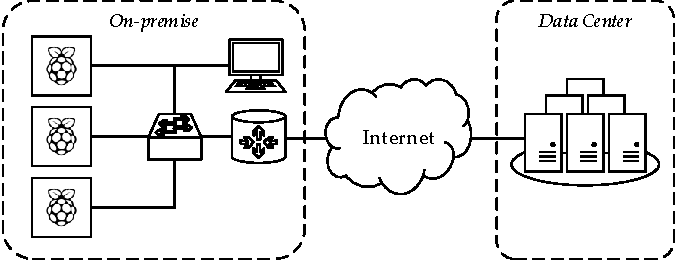
\includegraphics[width=0.8\textwidth]{figures/network-setup}
  \caption[Network topology of the experimental setup]{The experimental setup's network topology}\label{fig:network-topology}
\end{figure}
The test environment's network topology is depicted in \Cref{fig:network-topology}. The original testbed (``on-premise'') consists of three ARM-based SBCs (Raspberry Pi\footnote{\url{www.raspberrypi.org}} 3) whose network interfaces are connected by a Gigabit LAN switch (left-hand side in \Cref{fig:network-topology}). The three nodes represent on-board computing devices in a hypothetical vehicle. Furthermore, connected to the switch is also a workstation which fulfills the sole purpose of conducting the tests, \ie , it is not directly involved in the test execution per se. The local test environment is connected to the remote data center through a 100 Mbit/s broadband Internet connection.

Representative of the ``cloud'' in the tests is a single root server supplied by the cloud provider DigitalOcean\footnote{\url{www.digitalocean.com}} (right-hand side in \Cref{fig:network-topology}). To ensure realistic latency values, a server location was chosen that was in the vicinity of the test setup---but not too close. Considering its vicinity to Munich, Frankfurt (Main) was a suitable choice. The two cities are about 300 km away from each other (as the crow flies).

Throughout the whole study, the software composition remained unchanged. As DDS implementation OpenDDS\footnote{\url{www.opendds.org}} was chosen. The middleware was configured to utilize dynamic service discovery (without service repository) and RTPS over UDP as wire protocol. The optional Data Local Reconstruction Layer (DLRL), by which messages are converted into type safe data structures, was used. The overhead caused by this is evaluated and discussed in \Cref{sec:ddslatency}. Generally, default QoS settings were used for the tests, except in cases where a point was made to explicitly deviate from the defaults, \eg , the \liveliness\ settings in \Cref{sec:failovertest}. Moreover, all benchmark programs were developed in the C++ language to maximize their run-time performance.

Naturally, in the benchmarks concerned with the testing of \wnet , containers were connected by means of a \wnet\ overlay network. For the connection between all local nodes (on-premise), fast datapath forwarding mode was used. Due to the characteristics of the network between the local nodes and the cloud, fast datapath was not applicable for that connection. Consequently, local containers and cloud containers were connected via sleeve mode.
The detailed specifications of the involved computing nodes and the employed software are given in \Cref{tab:test-specs}
%
\begin{table}[H]
  \caption[Test environment specifications]{Test environment specifications}\label{tab:test-specs}
  \centering
  \begin{tabular}{p{0.235\textwidth} | p{0.335\textwidth}  p{0.335\textwidth}}
    \toprule
       & \textbf{On-premise} & \textbf{Remote} \\
    \midrule
    	Description & Raspberry Pi 3 Model B  & DigitalOcean 1 GB Droplet\\
    	Number of nodes & 3  & 1\\
    Theoretical network bandwidth & 100 Mbit/s (down), \newline 40 Mbit/s (up) & 40  Gbit/s (up- and down)\\
    	\midrule
    	Operating system & Raspbian GNU/Linux 9.3  & Ubuntu 16.04.3 LTS\\
    	Kernel & 4.9.59-v7+ w/ real-time patch \emph{PREEMPT\_RT} 4.4.9-rt17 & 4.4.0-112-generic \\
      CPU & ARMv7 rev 5  Quad Core (1.2 GHz) & Intel(R) Xeon(R) E5-2650 v4 Single Core (2.20GHz) x86\_64 \\
      Memory (RAM) & 1 GB & 1 GB  \\
      \midrule
      DDS & \multicolumn{2}{c}{OpenDDS 3.12.1}\\
      Docker  & \multicolumn{2}{c}{18.03.0-ce}\\
      \wnet & \multicolumn{2}{c}{2.2.1}\\
    \bottomrule
  \end{tabular}
\end{table}
%
%
%
%
%
%
%
%
%
%
\section{Benchmarks}

\subsection{Latency Benchmark} \label{sec:plainlatency}
\paragraph{Motivation.} An essential non-functional requirement for computer networks is responsiveness. Especially in real-time systems, where timing requirements must be met, it is vital that information exchange is performed in the fastest, most predictable way possible. A common metric for a network's responsiveness is latency. Latency is usually measured by the time it takes for a packet to be transmitted from one peer to another and back again. The unit of this measure is round-trip time (RTT), and is typically indicated in milliseconds.

To evaluate the aptitude of the presented system it is essential to consider the latency overhead that \weave\ overlay networks incur. Since the approach is intended to work over the Internet---and public networks are inherently insecure---encryption is vital. Thus, in addition to the overhead induced by the overlay network itself, the overhead caused by encryption is also of interest. Hence, tests are needed measuring latency not only of \emph{plain} overlay networks but also of \emph{encrypted} overlay networks.


\paragraph{Method.}

\begin{figure}[htpb]
  \centering
  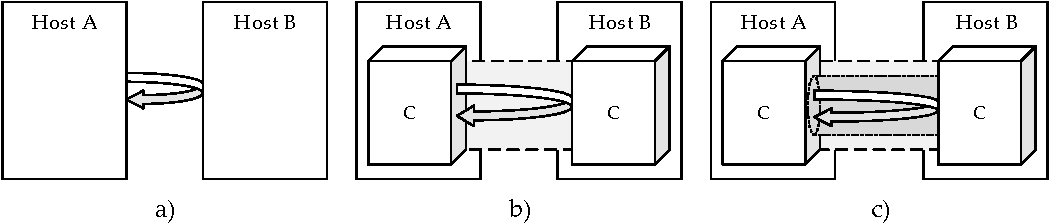
\includegraphics[width=\textwidth]{figures/ping-test}
  \caption[Latency experiment setup]{Latency experiment investigating three cases.
\begin{inparaenum}[a)]
  \item \experim{Plain}: two hosts connected without overlay network.
  \item \experim{Weave}: two containers connected via \wnet .
  \item \experim{Encrypted}: two containers connected via encrypted \wnet .
\end{inparaenum}
}\label{fig:latency-setup}
\end{figure}

In this test, latency was measured between two hosts connected over the Internet, both with, and without overlay-enabled container networking. To sample RTTs, a constant stream of ping messages was sent from one of the Raspberry Pis to the remote host and back. The Linux tool \emph{ping}, which pings hosts via ICMP\footnote{``Internet Control Message Protocol''} Echo Requests and Replies, was employed to take the measurements.

Three experiments were conducted, comparing the average latencies of
\begin{inparaenum}[(a)]
  \item plain host-to-host communication (``\experim{Plain}''),
  \item via \wnet\ (``\experim{Weave}''), and when employing
  \item encryption over \wnet\ (``\experim{Encrypted}'')
\end{inparaenum}
(\cf Figure \ref{fig:latency-setup}). The results from \experim{Plain} serve as the baseline for the two consecutive experiments. In each test run 3000 pings, each with a payload of 1 KB were transmitted. The sending peer would wait for the response of the previous message before sending another request. Thus, only one packet was in flight at a time.

\paragraph{Results.} \Cref{fig:latency-relative} depicts the results of the benchmark. The Y-values of the chart represent the average round trip time of the 3000 pings. Note that the Y-axis is cropped to the interval between 28 and 29 ms to emphasize the differences in the bars' heights. The results reveal that the latency overhead incurred by \wnet\ is very minor. In the case of plain host-to-host communication (\experim{Plain}), round trips took on average 28.4 ms. When sending the pings over a \weave\ overlay (\experim{Weave}), RTTs increased to an average of 28.6 ms, which is equivalent to an 0.9\% increase. Lastly, in the case of encrypted overlay networking (\experim{Encrypted}), the average RTTs reached a maximum of 29.0 ms---an increase of 2.1\% compared to \experim{Plain}.
\begin{figure}[htpb]
  \centering
  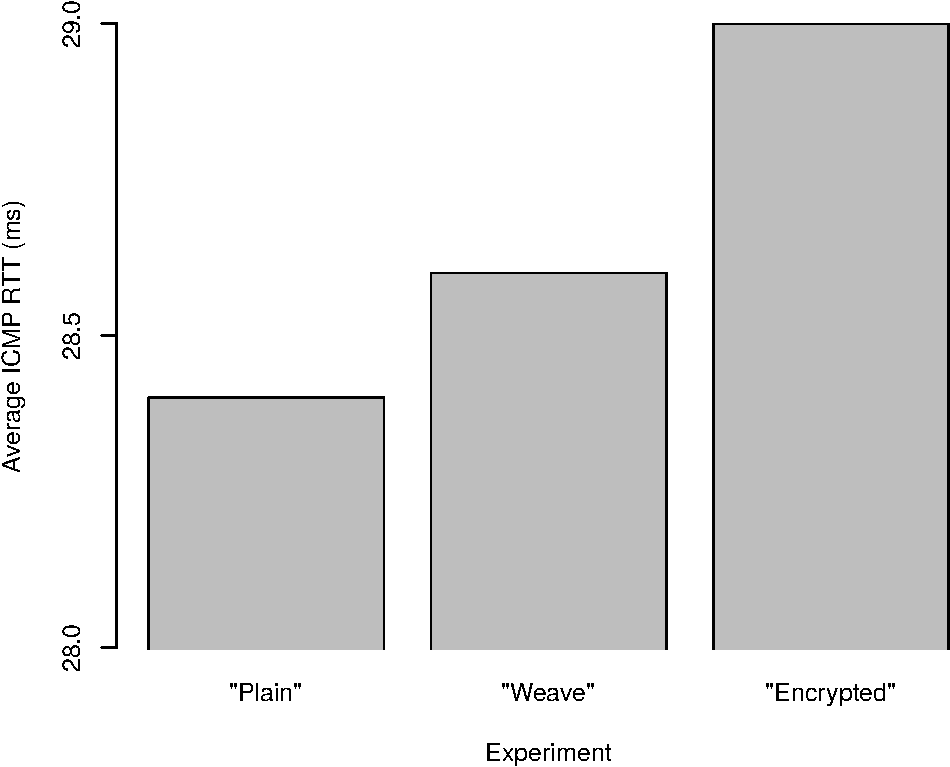
\includegraphics[width=0.45\textwidth]{figures/ping-bar}
  \caption[\weave\ latency experiment results]{Average round trip times in the scenarios \experim{Plain}, \experim{Weave}, and \experim{Encrypted}}\label{fig:latency-relative}
\end{figure}
%
%
%
%
%
%
%
%
%
%
\subsection{Throughput Benchmark} \label{sec:throughput}
\paragraph{Motivation.}
In modern vehicles, unprecedented amounts of data, originating from cameras, lidars and other sensors, is accumulated and distributed to the vehicle's various computing nodes. The presented approach allows scenarios in which that data is processed in the cloud. This prospect raises the question how well the approach can deal with such high volumes of data. In particular, the maximum theoretically achievable throughput is of primary interest. Throughput is a measure for how much data per time can be transmitted over a network. Since little data is available on \wnet 's throughput performance, according benchmarks were carried out.

\paragraph{Method.} To measure throughput, the tool \emph{iperf3}\footnote{\url{www.iperf.fr}} was used. iperf continuously sends data from one node to another over a TCP/IP connection. From the volume of the transmitted data and the duration of the transmission, the effective network throughput can be calculated. In each test run iperf would continuously send as much data as possible within a timeframe of 60 seconds. As in the previous test, three scenarios were tested:  \experim{Plain}, \experim{Weave}, and \experim{Encryped}. Explanations of these scenarios can be found in the description of the previous test.

A fact to consider is that routing packets over overlays is computationally expensive---even to the extent that at a certain point the CPU may become the bottleneck of the operation. In other words, network throughput may hit a boundary incurred by insufficient computing resources, even though the networking capacity is not entirely exhausted. This experiment investigates the case where enough computing resources are available, such that the network channel's capacity is the limiting factor. The case where the CPU's performance is insufficient is investigated in the experiment after this one (\cf \ref{sec:utilization}).

\paragraph{Results.}
The results of this benchmark are depicted in \Cref{fig:throughput}. The results show that unencrypted \wnet\ (\experim{Weave}) slightly reduces throughput performance when compared to \experim{Plain} scenario (5\% reduction). When furthermore encryption is applied to the overlay network (\experim{Encrypted}), an additional throughput impairment can be observed. Overall, encryption incurs an overhead of 6.7\% compared to the \experim{Plain} scenario. These values can be considered decent. Once more, it shall be noted that in this case enough computational resources were available. \Ie , the CPU was not fully utilized but the network channel was at its limits.
\begin{figure}[htpb]
  \centering
  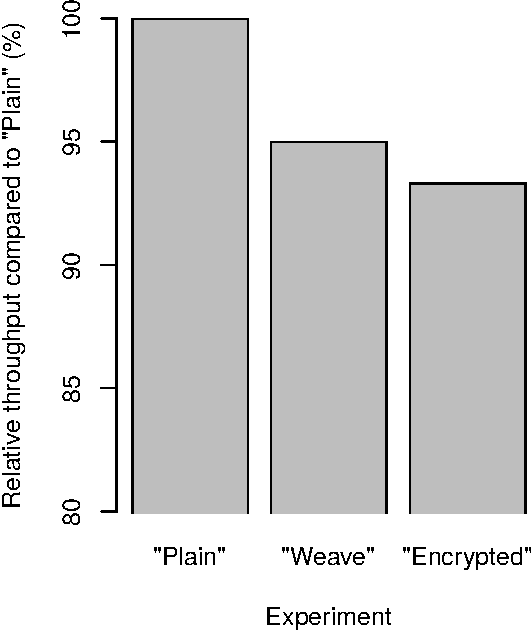
\includegraphics[width=0.4\textwidth]{figures/throughput}
  \caption[\weave\ throughput benchmark results]{Relative throughput in the scenarios \experim{Plain}, \experim{Weave}, and \experim{Encrypted}}\label{fig:throughput}
\end{figure}
%
%
%
%
%
%
%
%
%
%
\subsection{Resource Utilization Test} \label{sec:utilization}
\paragraph{Motivation.} The routing of data packets through an overlay puts significant load on the host's CPU. Under circumstances, the transmission of data, which is typically an IO-bound operation, might become CPU-bound. In this situation the CPU becomes the bottleneck of the operation. In embedded systems, in which computing resources are limited, this might be problematic. Hence, an experiment was designed aimed to investigate the impact of overlays on CPU utilization.

\paragraph{Method.} In this experiment, sample data was sent from a Raspberry Pi to the remote host via iperf (\cf \Cref{sec:throughput}) over an encrypted \wnet\ overlay. During the time of data transmission, CPU utilization was measured using the Linux tool \emph{sar}. 25 test runs were conducted using different bandwidth settings: bandwidth was gradually increased in 1 Mbit/s increments, starting at 1 Mbit/s, and ending in 25 Mbit/s. This bandwidth will be called \emph{target bandwidth} in the following. The target bandwidth is an artificially imposed upper bound and may differ quite substantially from the bandwidth that is actually achieved. The achieved bandwidth will be called \emph{observed bandwidth}, or \emph{throughput}.

\paragraph{Results.}
\Cref{fig:cpu} depicts the test results. In the diagram, each data sample represents the average CPU utilization of the sending node during a particular test run. The Y-axis represents the overall CPU utilization of the sending machine (Raspberry Pi), and includes the cumulative load of all programs running on the system. Hence, the measurements include a bit of noise. The dashed horizontal line indicates the maximum load of a single core in a quad core CPU.
\begin{figure}[htpb]
  \centering
  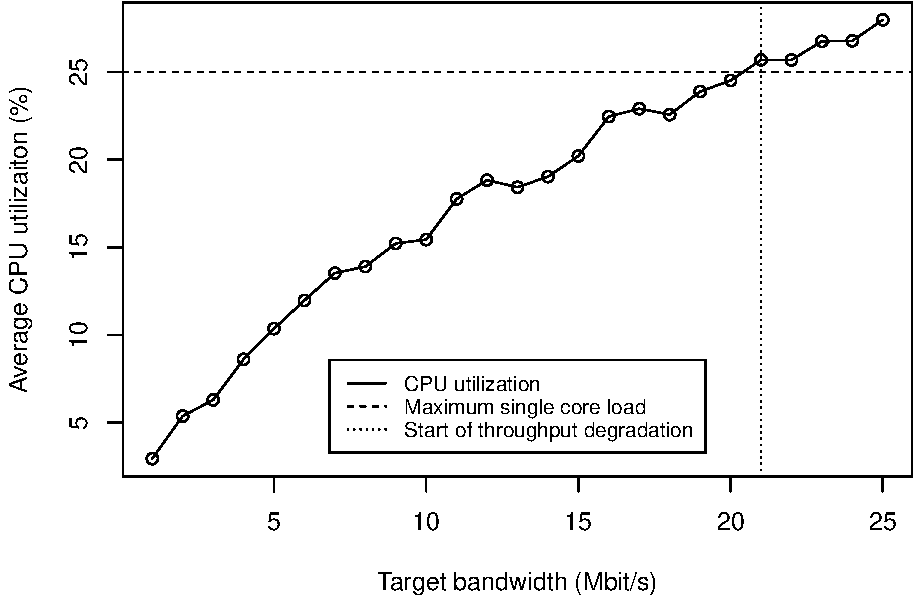
\includegraphics[width=0.73\textwidth]{figures/cpu}
  \caption[\weave\ CPU utilization test results]{In \weave\ overlays, CPU utilization increases linearly with network throughput. At around 21 Mbit/s, the test node reaches a computational limit (one of the four cores is fully utilized) such that the effective throughput stagnates (not displayed).}\label{fig:cpu}
\end{figure}

The results show that CPU utilization increases linearly with the target bandwidth. What is striking is that the point of full resource utilization of a single core is reached quite early, at around 21 Mbit/s target bandwidth (dotted vertical line). \wnet\ is a single-threaded program, and as such, experiences performance stagnation once the core it runs on is fully occupied. At this point, first throughput degradations become evident, so that the setup begins to fall short on delivering the desired bandwidth. The maximum observed bandwidth that the setup could achieve over numerous test runs was 23.6 Mbit/s.
However, the maximum (theoretically) achievable throughput in the test setup was 100 Mbit/s. Thus, a large part of the network's capacity was left unused. This circumstance is a strong evidence that a CPU-bound wall was hit.
%
%
%
%
%
%
%
%
%
%

\subsection{DDS Latency Benchmark} \label{sec:ddslatency}

\paragraph{Motivation.} So far, all experiments were concerned with \wnet\ exclusively and did not involve DDS. To the best of the author's knowledge, there are no empirical studies yet on how well DDS performs in VXLAN-based overlay networks spanning over the Internet. Hence, benchmarks were conducted to evaluate latency overhead incurred by DDS in such scenarios.

\paragraph{Method.} The method of this experiment is similar to the previous latency experiment (section \ref{sec:plainlatency}) in that the RTT between two hosts connected over the Internet are used as the measure of latency. Two cases are investigated:
\begin{inparaenum}[(i)]
	\item RTTs via ICMP ping, and
	\item RTTs via DDS ping.
\end{inparaenum}
For the former case, the ICMP ping results from the previous latency experiment are used. These results serve as a reference point to which DDS is compared to. In order to measure DDS RTTs, a ping application was developed that functions similar to classic ping: a message containing a recent timestamp ($T_1$) is sent from one endpoint ($A$) to another ($B$) via a topic named ``ping'', and the same message is then sent back to $A$ without modifications. The returned message is published on a topic named ``pong'', which $A$ is subscribed to. Upon reception of the returned message, $A$ creates a reception timestamp ($T_2$) and subtracts that timestamp from $T_1$, effectively calculating the RTT. This process is then repeated multiple times. Between the reception of a returned message and the dispatch of the next message, the sender was configured to wait for a few milliseconds to make sure that only a single message was in circulation at any time.

Of course, sending data via DDS entails a lot more than simple ICMP pings, like \eg\ the marshaling and parsing of messages. The comparison with ICMP is therefore a very ambitious one. As ICMP pings require very little processing, the largest part of the measured round trip time accounts for pure message transmission. ICMP ping is therefore a good reference point to measure the overhead induced by DDS, and in particular, RTPS.

The tests in both cases (ICMP an DDS) were performed in an encrypted \wnet\ overlay network (``\experim{Encrypted}'') to ensure practical experiment conditions. Both times, ping messages carried a payload of 1 kB. The results presented below are the average values calculated from 300 pings.


\paragraph{Results.}
The results of the benchmark are presented in \Cref{tab:dds-latency}. The overhead incurred by DDS, when compared to ICMP ping, is in the 15-to-18 per cent range. The overhead can be explained by the fact that DDS does a lot more than just transmit data from point to point. Most notably, the enforcement of certain QoS policies takes their toll on latency, as well as the marshaling, serialization and parsing of message payloads by the DLRL. Considering this, the overhead of DDS can be considered reasonable.

\begin{table}[H]
  \caption[DDS latecy benchmark results]{DDS latency benchmark results: ICMP and DDS round-trip-times}\label{tab:dds-latency}
  \centering
  \begin{tabular}{p{0.2\textwidth} | p{0.2\textwidth} p{0.2\textwidth} | p{0.2\textwidth}}
    \toprule
       & \textbf{ICMP} & \textbf{DDS} & \textbf{DDS Overhead} \\
    \midrule
    	Minimum & 24.32 ms & 28.05 ms & +15.36 \%\\
    	Average & 27.00 ms & 30.84 ms & +14.27 \%\\
    	Maximum & 47.36 ms & 55.96 ms & +18.16 \% \\
    	$\sigma$ & 1.75 ms & 2.39 ms &\\
    \bottomrule
  \end{tabular}
\end{table}
% The results of the benchmark are presented in \Cref{fig:dds-latency}. With the experiment it was shown that DDS adds reasonable overhead when compared to the plain transmission time of ICMP ping. The overhead ranged between 11.45\% at min, and 17.55\% at max. On average, the overhead was at 14.74\%. The overhead can be explained by the fact that DDS does a lot more than just transmit data. Most notably, the enforcement of certain QoS policies took their toll on latency, as well as the marshaling, serialization and parsing of message payloads by the DLRL.
%\begin{figure}[htpb]
%  \centering
%  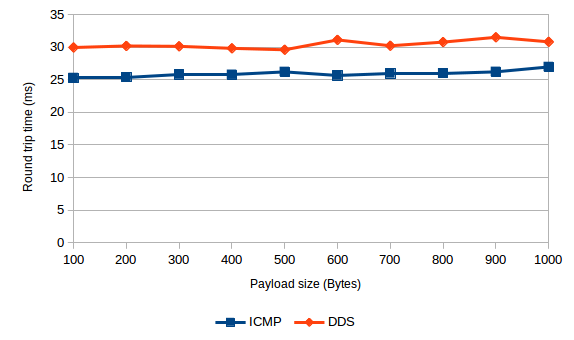
\includegraphics[width=0.7\textwidth]{figures/dds-latency}
%  \caption[DDS latency benchmark results]{The average RTT of differently sized packets when using DDS versus ICMP}\label{fig:dds-latency}
%\end{figure}
%
%
%
%
%
%
%
%
%
%
\subsection{Failover Test}\label{sec:failovertest}
\paragraph{Motivation.} The presented approach allows for many innovative usage scenarios. For instance, consider the following situation: A service running on an on-board computer within a vehicle suddenly fails, \eg\ due to a hardware defect. As a reaction, a fallback service needs to take over. Consider now that the fallback service is not running on another on-board computer but within the cloud. Through DDS QoS policies, a failover mechanism can be realized (\cf \ref{sec:failover}) which allows for a quick transition to the remote backup service. An interesting question is how long the whole failover process, \ie\ switching to a backup service in case of failure, takes in a cloud scenario.

\newcommand{\proda}{$S\textsubscript{A}$}
\newcommand{\prodb}{$S\textsubscript{A*}$}
\newcommand{\cons}{$S\textsubscript{B}$}

\paragraph{Method.} To test the performance of DDS's failover qualities an experiment was designed to replicate a scenario in which a service fails so that another, remote service must take over. In the test scenario there are three services: two services which continuously produce data (\proda , \prodb) in the interval $t_i$, and one which consumes the data (\cons). \proda\ has precedence over \prodb\ (\ie\ it possesses a higher \ownership\ value) and is therefore the ``main supplier'', while \prodb\ is considered the ``backup supplier''. \proda\ and \cons\ are both deployed two on separate Raspberry Pis (representative of two ECUs in a vehicle), and \prodb\ is running in the cloud. A schematic of the experiment is depicted in \Cref{fig:failover}. It shall be noted that, contrary to what the figure suggests, communication is not point-to-point, but topic-based. \proda\ as well as \prodb\ publish data samples on the same topic and \cons\ is subscribed to that topic.
\begin{figure}[htpb]
  \centering
  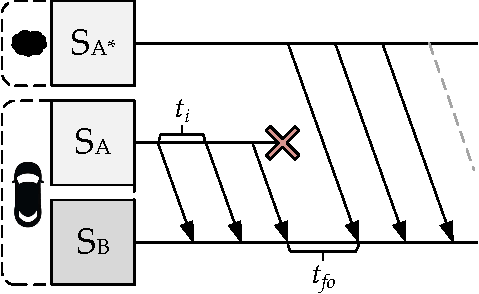
\includegraphics[width=0.5\textwidth]{figures/takeover}
  \caption[Failover experiment schematic]{Failover scenario: vehicular service \proda\ fails to supply \cons\ with data so that cloud-based service \prodb\ must take over}\label{fig:failover}
\end{figure}

In the process of sending data, a failure of \proda\ is simulated by abruptly shutting down the application process (indicated by the cross in the image). In this event, the cloud-based backup service, \prodb , needs to take over. To determine the effective failover time, $t_{fo}$, the time between the last message from \proda\ and the first message from \prodb\ is measured. The failover is performed implicitly by DDS through the failover mechanism described in \Cref{sec:failover}. In this experiment, \liveliness\ is set to 100 ms, indicating that after 100 ms of inactivity, a service is declared ``dead''. The experiment is performed on an encrypted Weave overlay (case ``\experim{Encrypted}'').

%%% Setup
% Pub1: docker run -ti --rm --entrypoint /bin/bash kugele1337/spammer-pub-qemu
% Pub2: docker run -ti --rm --entrypoint /bin/bash kugele1337/spammer-pub
% Sub: docker run --rm -ti  --entrypoint /bin/bash -v $(pwd)/results:/opt/workspace/results kugele1337/spammer-sub-qemu

%%% Execute
% Pub1: ./publisher -DCPSConfigFile rtps.ini --samples 9999999 --delay 80 --failafter 99999999 --liveliness 100 --payload a
% Pub2: ./publisher -DCPSConfigFile rtps.ini --samples 10000000999 --delay 80 --liveliness 100 --payload bb
% Sub: ./subscriber -DCPSConfigFile rtps.ini --debug --liveliness 100 --filename-fail 100liveliness-80delay19.csv

\paragraph{Results.} In 100 test runs, an average $t_{fo}$ of 131.3 ms was measured. The fastest failover took 103.2 ms, and the slowest one took 181 ms. Of course, the \liveliness\ settings heavily influence the failover times as \liveliness\ determines how fast a failure is detected. After subtracting the 100 ms needed for failure detection, the resulting figures may be considered reasonable.
%
%
%
%
%
%
%
%
%
%
%
%
%
%
%
%
%
%
%
%
